\documentclass[french]{article}
 
\usepackage[utf8]{inputenc}
\usepackage[T1]{fontenc}
\usepackage{babel}
\usepackage{graphicx}
\usepackage{amsmath}
\usepackage{caption}

\begin{document}
\section{Introduction}
\begin{figure}[ht]
	\centering
	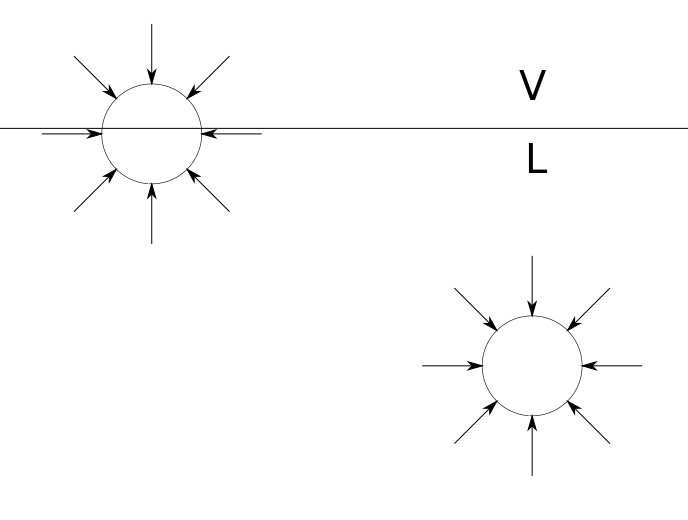
\includegraphics[scale = 0.3]{./image/rondforces.png}
	\caption{Ligne triple}
\end{figure}

La tension de surface est une force par unité de longueur.\\ 

Dans un liquide ayant une interface, une molécule complètement immergée dans le liquide est soumise à des forces d'interactions avec les autres molécules (du liquide) dans toutes les directions. 

Une molécule située à l'interface, la somme des interactions (avec les molécules du même fluide) est non nulle est dirigée vers l'intérieur du liquide. Il existe donc une force supplémentaire qui permet de maintenir l'interface.

Cette force supplémentaire (par unité de longueur) est la tension de surface.\\



la tension de surface est aussi une énergie par unité de surface, c'est l'énergie (par unité de surface) pour séparer les interfaces et les envoyer à l'infini l'une par rapport à l'autre.


\subsection{Mouillage}
Le mouillage est l'action de mouiller et mouiller consiste à  mettre en contact avec un liquide.\\


C'est le paramètre d'étalement $S = \gamma_{SV} - (\gamma_{SL} + \gamma_{LV}) = \gamma_{LV}(\cos\theta_{E} - 1)$ qui caractérise le mouillage lorsque la goutte est en équilibre sur un support matériel.

Quand $S > 0$, on parle de mouillage total et quand $S < 0$, on parle de mouillage partiel.\\

Nous nous intéressons en particulier à une goutte dont le support est une plaque plane dans les conditions de mouillage partiel. 
\begin{figure}[ht]
	\centering
	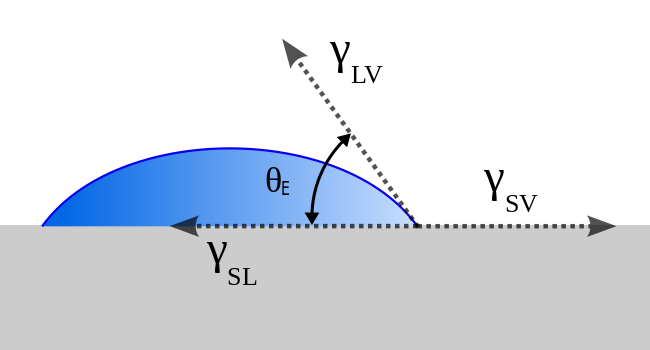
\includegraphics[scale = 0.3]{./image/Contact_angle2.png}
	\caption{Ligne triple}
\end{figure}



Le substrat est le nom donné au support (solide ou liquide) sur lequel la goutte de liquide repose.

Lorsqu'une goutte d'eau est posée sur support solide, il y a formation de 3 interfaces et donc de 3 tensions de surface.


En projetant les tensions de surface sur l'horizontale on obtient :

\begin{equation}
	\label{eq:Young}
	\gamma_{SV}  = \gamma_{SL} + \gamma_{LV}\cos\theta_{E}
\end{equation}

C'est la loi de Young.

\section{Hystérésis}


Dans la réalité l'angle statique $\theta_{E}$ n'est pas unique et on a :


\begin{equation}
	\theta_{E,r} <= \theta_{E} <= \theta_{E,a}
\end{equation}

Lorsque l'angle de contact $\theta$ vérifie $\theta < \theta_{E,r}$, la goutte se met à reculer et l'angle de contact $\theta$ à l'arrière de la goutte est appelé $\theta_{r}$.\\

Lorsque l'angle de contact $\theta$ vérifie $\theta_{E,a} < \theta$, la goutte se met à avancer et l'angle de contact $\theta$ à l'avant de la goutte est appelé $\theta_{r}$.\\

Dans le cas d'un surface parfaite $\theta_{a}$ et $\theta_{r}$ sont égaux.\\

L'hystéréris (en parlant d'angle de contact) est la différence $\theta_{a}-\theta_{r}$ puisque $\theta_{a}$ et $\theta_{r}$ ne sont égaux en pratique.

\section{Modèles d'angle dynamique}

L'angle de contact de la goutte en mouvement (l'angle dynamique) est différent de l'angle de contact quand la goutte es équilibre (angle statique).



Les grandeurs que nous avançons mesurées expérimantalement en prenant les photos d'une goutte d'eau dans la soufflerie sont l'angle avant $\theta_{a}$, l'angle arrière et 



\begin{figure}[ht]
	\centering
	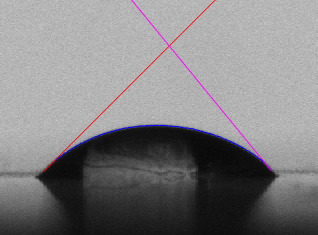
\includegraphics[scale = 0.6]{./image/crop_tvitesse=28_volume=003.png}
	\caption{Goutte d'eau de volume $0.03$ml avec $\theta_{a} = 45^{o}$ et $\theta_{r} = 50.17^{o}$}
\end{figure}

\begin{figure}[ht]
	\centering
	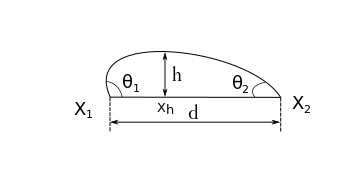
\includegraphics[scale = 1]{./image/rrgou2.png}
	\caption{Paramètres mesurés}
\end{figure}

\begin{itemize}
\item $U$ vitesse de la goutte, $\theta(U)$?
\item Le nombre capillaire : $C_{a} = \frac{\text{effets visqueux}}{\text{effets capillaires}} = \frac{\eta U}{\gamma}$
\item De Gennes : $ \theta \left(\theta^{2} - \theta_{s}^{2}\right) = \pm 6\ln\left(\frac{b}{a}\right)C_{a}$
\item Cox et Voinov : $\theta^{3} - \theta_{s}^{3} = \pm 9\ln\left(\frac{b}{a}\right) C_{a}$
\item Cinétique moléculaire: $\left(\theta^{2} - \theta_{s}^{2}\right) = \frac{\nu NkT}{2\pi fL_{m}h}C_{a}$
\item Linéaire : $\theta - \theta_{s} \propto \pm U$
\end{itemize}

\end{document}
